The Groundwater Transport (GWT) Model \citep{modflow6gwt} in \mf represents the mass of solute in a cell as the sum of a dissolved part, held in the water in the cell, and a sorbed part, held on the solid aquifer material. Both parts are multiplied by the water saturation, $S_w$, in the storage terms on the left side of equation~\ref{eqn:gwtpde} of Chapter~\ref{ch:sorption},

\begin{equation}
\label{eqn:strandstorage}
\frac {\partial \left ( S_w \theta_m C \right )}{\partial t}
+ \hat{f}_m \rho_{b,m} \frac {\partial \left ( S_w \overline{C} \right ) }{\partial t} ,
\end{equation}

\noindent where $S_w$ is the water saturation ($L^3/L^3$), $\theta_m$ is the mobile-domain effective porosity ($L^3/L^3$), $C$ is the mobile-domain volumetric concentration of solute ($M/L^3$), $\hat{f}_m$ is the volume fraction of the mobile domain ($L^3/L^3$), $\rho_{b,m}$ is the bulk density of aquifer material in the mobile domain ($M/L^3$), and $\overline{C}$ is the concentration of sorbate ($M/M$).

Because the sorbed term is multiplied by $S_w$, the sorbate in a cell is proportional to the saturated part of the cell. When the water table falls and $S_w$ decreases, the sorbed mass of the cell decreases with it, and the sorbate that the cell gives up is returned to the water that remains. Mass is conserved, but the sorbate is redissolved into a smaller volume of water and the simulated concentration rises. The solid aquifer material does not drain, and the sorbate on it does not move with the water table, so the rise in concentration is an artifact of the storage term rather than a physical process. Approximations in the treatment of changes in fluid storage during transient flow are described by \citet{goode1990, goode1992}.

Two quantities of solute are affected, and figure~\ref{fig:strandedmassconcept} shows what becomes of each. When the water table falls, the sorbate of the drained interval is released to the water that remains, and the concentration rises. The volume of water in the mobile domain is the saturation times the porosity times the volume of the cell, so the drained interval is treated as holding no water at all. Whenever the specific yield is less than the porosity, the drained interval keeps some of its water, the retained water, and the mobile water volume of the cell changes by more than the water the flow model releases from storage. The solute in the retained water is not carried into the next time step, and mass is lost. When the water table rises, the interval is saturated again as though it had held water at the concentration of the previous time step, and mass is created. The two do not cancel over a cycle unless the cell returns to the same saturation at the same concentration.

\begin{figure}[!ht]
	\begin{center}
	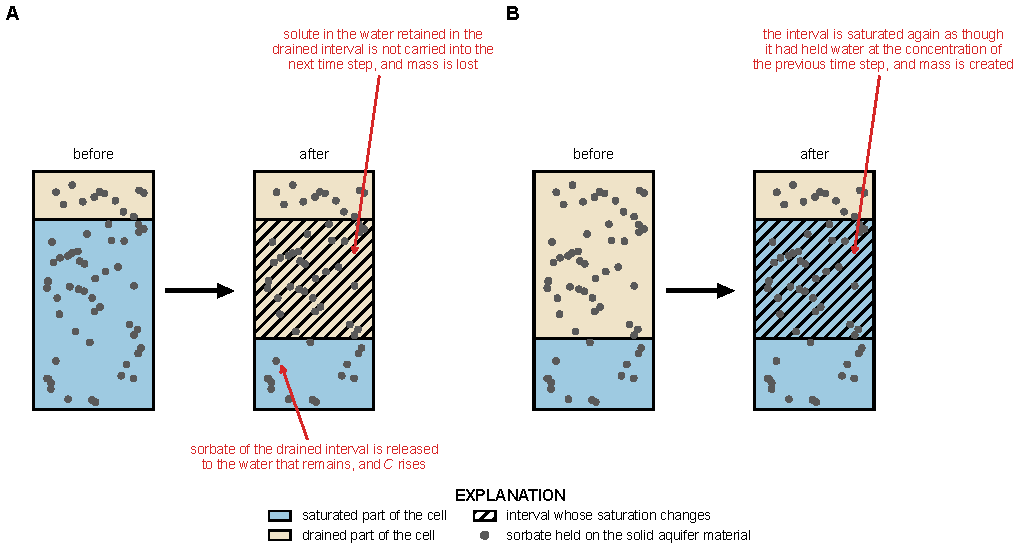
\includegraphics{./Figures/MSTStrandedMassConcept.pdf}
	\caption[Diagrams showing what becomes of the solute of a cell whose water table moves]{Diagrams showing what becomes of the solute of a cell whose water table moves, without the stranded mass option. \textit{A}, The water table falls, the saturated volume decreases, the sorbate of the drained interval is released to the water that remains and the concentration rises, and the solute in the retained water of that interval is not carried into the next time step, so mass is lost; \textit{B}, the water table rises, the saturated volume increases, and the interval is saturated again as though it had held water at the concentration of the previous time step, so mass is created}
	\label{fig:strandedmassconcept}
	\end{center}
\end{figure}

The STRANDED\_MASS option of the Mobile Storage and Transfer (MST) Package holds both quantities out of the mobile domain when a cell drains, and returns them when the cell rewets. This chapter describes the formulation, shows its effect for a cell with an oscillating water table, and assesses what the formulation does and does not represent.

\subsection{Formulation}

A cell that uses the option holds its stranded mass in two reservoirs, one for the solute of the retained water and one for the sorbate. Stranded mass is a mass rather than a concentration, and it is immobile: it is not advected, it takes no part in dispersion, and it is not transferred between cells. Mass moves between the mobile domain and the reservoirs only in matched pairs, so the sum of the two is conserved by construction.

\subsubsection{Drainage}

Over a time step in which the saturation of a cell decreases, two quantities of solute stay behind. The first is the solute in the retained water. The mobile water volume of a cell is $S_w \theta_m V_{cell}$, so it changes by $\Delta S_w \theta_m V_{cell}$, but the flow model releases from storage only the drainable part of the pore space. The difference is the retained water,

\begin{equation}
\label{eqn:strandretained}
V_{r} = \Delta S_w \, \theta_m \, V_{cell} - V_{s} ,
\end{equation}

\noindent where $V_{r}$ is the retained water volume ($L^3$) and $V_{s}$ is the volume of water released from storage over the time step ($L^3$), which for an unconfined cell is the specific yield times the change in head times the area of the cell. The retained water volume is not a new input; it follows from the porosity of the transport model and the specific yield of the flow model, and it is set to zero if those two would make it negative. The second quantity is the sorbate of the drained interval, because the solid aquifer material does not drain. The mass moved out of the mobile domain and into the reservoirs is

\begin{equation}
\label{eqn:strandrate}
\Delta M_{st} = V_{r} \, C + \Delta S_w \, V_{cell} \, \hat{f}_m \rho_{b,m} \overline{C} ,
\end{equation}

\noindent where $\Delta M_{st}$ is the mass added to the stranded mass over the time step ($M$), $\Delta S_w$ is the decrease in saturation over the time step ($L^3/L^3$), and $V_{cell}$ is the volume of the cell ($L^3$). The first term on the right side of equation~\ref{eqn:strandrate} is the solute in the retained water, which the storage term of the mobile domain no longer carries once the water table has fallen below it. The second term is the sorbate that the storage term would otherwise have released, so the two cancel and none of the sorbate that the cell gives up reaches the water that remains.

The concentrations in equation~\ref{eqn:strandrate} are those at the end of the time step, the same concentrations used for the storage of sorbate, so the sorbate held back is the sorbate that the storage term releases for any of the sorption isotherms of the MST Package.

\subsubsection{Rewetting}

The mass in each reservoir is taken to be distributed uniformly through the part of the cell that drained while mass was added to it. Each reservoir carries, in addition to its mass, the accumulated drained fraction $F$ that its mass represents; $F$ increases by $\Delta S_w$ each time the cell drains and mass is added to the reservoir, and decreases by the increase in saturation each time the cell rewets. A drainage that adds nothing to a reservoir, because the water held no solute or, for the aqueous reservoir, because no water was retained, does not extend the part that the reservoir represents, so mass held by a later drainage returns as soon as the part it came from rewets. Over a time step in which the saturation increases by $\Delta S_w'$, the mass returned to the mobile domain from each reservoir is

\begin{equation}
\label{eqn:strandreturn}
\Delta M_r = M_{st} \, \min \left ( \frac{\Delta S_w'}{F}, 1 \right ) ,
\end{equation}

\noindent where $\Delta M_r$ is the mass returned over the time step ($M$) and $M_{st}$ is the mass that the reservoir holds at the start of the time step ($M$). The returned mass enters the cell as a source of solute over the time step.

Measuring the returned share relative to $F$, rather than to the unsaturated part of the cell, makes returning the exact inverse of stranding. A cell that drains and then rewets by the same amount recovers all of the mass it gave up, and a cell that rewets part of the way recovers the corresponding share, because the mass of the part that remains drained stays there. The mass that returns is the mass that the same cell gave up; no neighboring cell is used, and no mass is created or discarded.

\subsubsection{Decay}

Each reservoir decays at the first-order rate given for its phase: the solute of the retained water at the rate for the dissolved phase, $\lambda_1$, and the sorbate at the rate for the sorbed phase, $\lambda_2$. The mass that a reservoir loses over a time step is

\begin{equation}
\label{eqn:stranddecay}
\Delta M_d = M_{st} \left ( 1 - e^{-\lambda \Delta t} \right ) ,
\end{equation}

\noindent where $\Delta M_d$ is the mass lost to decay over the time step ($M$) and $\lambda$ is $\lambda_1$ or $\lambda_2$ ($1/T$). A negative rate is production, following the convention used for the decay rates of the mobile domain, and because production is proportional to the mass held, a reservoir that holds no mass produces none. Zero-order decay is not applied to the stranded mass, because a zero-order rate would drive an empty reservoir negative; a warning is issued if zero-order decay is active.

\subsubsection{Budget}

Three quantities change the stranded mass of a cell,

\begin{equation}
\label{eqn:strandbalance}
\frac{d M_{st}}{d t} = \frac{\Delta M_{st}}{\Delta t} - \frac{\Delta M_r}{\Delta t} - \frac{\Delta M_d}{\Delta t} .
\end{equation}

The first two terms are transfers, exactly paired with the mobile domain, and are reported together as a single entry, STORAGE-STRANDED, in the model budget. Decayed stranded mass leaves the simulation without passing through the mobile domain, so reporting it in the model budget would add an outflow with no matching change in the mobile domain and drive the percent discrepancy away from zero. It is reported instead in a budget for the package, together with the storage of the stranded mass and the transfer with the mobile domain, in the same way that the Immobile Storage and Transfer (IST) Package reports the budget of an immobile domain. Decayed stranded mass never returns to the mobile domain; decay reduces the mass available to return later.

The stranded mass of every cell is saved to a file when the STRANDED FILEOUT option is used, in the same way that the sorbate concentration is saved with the SORBATE FILEOUT option, and a time series for one cell is obtained from that file. Neither quantity is available as an observation in the Observation (OBS) utility.

The stranded mass of a cell and the transfers reported in the budget are calculated from the same quantities at the end of each time step, so the two always agree.

\subsubsection{Saturation at the end of the previous time step}

The changes in saturation in equations~\ref{eqn:strandretained} through~\ref{eqn:strandreturn} are changes in the position of the water table in the cell, so the saturation at the end of each time step is recorded and used in the next. Without the option, the transport model infers the saturation at the end of the previous time step from the water released from storage, which gives the position of the water table only when the specific yield equals the porosity of the mobile domain; for the storage of sorbate, the inferred saturation omits the porosity altogether. With the option, both storage terms use the recorded saturation, so the mass held back cancels the mass that the storage terms release and the percent discrepancy of the model budget stays at zero.

Mass is stranded from the first time step. When the flow model is solved in the same simulation, the saturation at the start of the simulation is calculated from the initial heads in the same way that the flow model calculates it for convertible cells, confined cells, and the Newton formulation, so a simulation that begins with a large change in the water table needs no initial stress period with a stationary water table.

A transport model that reads the flows saved by a separate flow simulation does not have the saturation at the start of the simulation, because the saved flows begin at the end of the first time step. Such a simulation strands no mass during the first time step and writes a warning to the simulation listing file if the water table moved or a cell was dry at the end of the time step, since the saved flows do not show whether that cell drained; it should begin with a short stress period during which the water table does not move.

\subsubsection{Cells that drain completely}

A cell whose water table falls below its bottom is inactive for transport until it is rewet. Its reservoirs are not emptied: the mass they hold decays at the rate given for its phase and is returned when the cell is rewet, in proportion to the part of the drained interval that resaturates. The saturation of the cell is recorded while it is inactive, so the time step in which it becomes active again is treated as rewetting. Without that record, the saturation from before the cell went dry would stand, and a cell that returns wetter than it was when it went dry, but not full, would appear to have drained further and would strand mass instead of returning it.

\subsection{Extension to Immobile Domains}

An immobile domain represented with the IST Package multiplies its mass by the water saturation in the same way that the mobile domain does, so an immobile domain also returns its solute to the water that remains when a cell drains. Stranding is a property of a domain rather than of a cell: a simulation with $nim$ immobile domains would require $nim + 1$ sets of reservoirs, one for the mobile domain and one for each immobile domain, because each domain has its own bulk density, sorption parameters, and decay rates.

The formulation in this chapter is written in terms of the properties of a single domain, so stranding the mass of an immobile domain would use equations~\ref{eqn:strandrate} through~\ref{eqn:stranddecay} with the parameters of that domain, and would report the transfer with the mobile domain in the budget of the IST Package.

Immobile domains are not supported in the present version. Specifying STRANDED\_MASS together with an active IST Package is an error rather than a warning, because a simulation in which the mobile domain holds its sorbate back while the immobile domains continue to release theirs is harder to interpret than one in which neither does. The transfer of mass between the mobile and immobile domains needs no change, because it is already multiplied by the saturation and goes to zero as a cell dries.

\subsection{Example: Oscillating Water Table}

The effect of the option is shown for a single cell whose water table rises and falls. The cell is 100 by 100 meters (m) in plan, extends from an elevation of 40 \si{\meter} to an elevation of 0 \si{\meter}, and has a mobile-domain porosity of 0.3 and a specific yield of 0.15, so that half of the pore space drains and half is retained. A constant head in the cell next to it varies sinusoidally with a period of 100 days (d) about a mean of 24 \si{\meter} with an amplitude of 14 \si{\meter}, so that the saturation of the cell varies between about 0.25 and 0.95 over four cycles (fig.~\ref{fig:strandedmasshead}). The initial concentration is 100 grams per cubic meter (g/m$^3$) throughout, water entering through the constant head has a concentration of zero, and water leaving through it has the concentration of the cell it leaves. Advection and dispersion are not simulated, so no solute passes between the two cells and the storage terms are the only process that can change the solute mass of the tested cell. Solute leaves the simulation only through the constant head, and only from the cell that contains it. Where sorption is active it is represented with a linear isotherm using a bulk density of 1,600 kilograms per cubic meter (kg/m$^3$) and a distribution coefficient of $1 \times 10^{-4}$ cubic meters per kilogram (m$^3$/kg); where decay is active, the first-order rate is 0.005 \si{\per\day} for both the dissolved and the sorbed phase. A time step of 1 \si{\day} is used throughout, and the water table is held still during the first stress period.

\begin{figure}[!ht]
	\begin{center}
	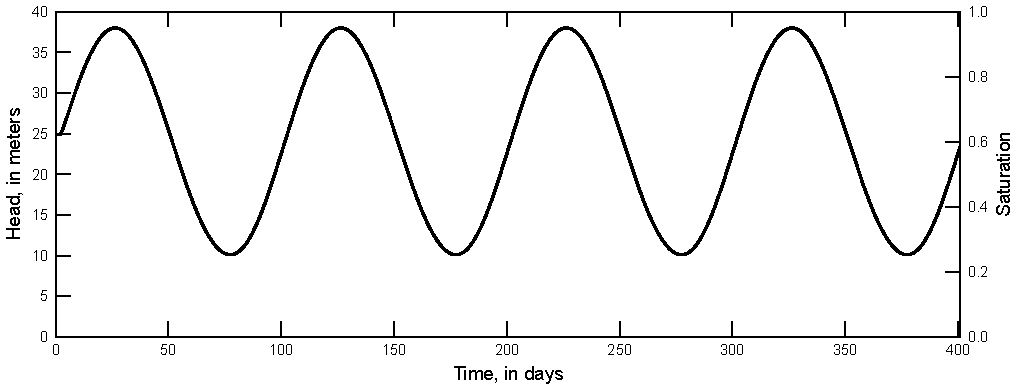
\includegraphics{./Figures/MSTStrandedMassHead.pdf}
	\caption[Graph showing the simulated head and water saturation for the oscillating water table example]{Graph showing the simulated head in the tested cell and the corresponding water saturation for the oscillating water table example. The cell extends from an elevation of 40 meters (m) to an elevation of 0 \si{\meter}, and the constant head in the cell next to it varies sinusoidally with a period of 100 days (d) about a mean of 24 \si{\meter} with an amplitude of 14 \si{\meter}}
	\label{fig:strandedmasshead}
	\end{center}
\end{figure}

Simulated concentrations rise as the cell drains in every case, because the water that remains occupies a smaller volume. Without sorption or decay (fig.~\ref{fig:strandedmassnosorption}\textit{A}), the peak concentration reaches 163 g/m$^3$ without stranded mass and 126 g/m$^3$ with it, a reduction of 23 percent, because the solute in the retained water is held out of the mobile domain instead of being carried by the water that remains.

The solute mass of the tested cell (fig.~\ref{fig:strandedmassnosorption}\textit{B}) shows the effect more directly than the concentration does, because a concentration reflects both the mass in the cell and the volume of water that holds it. No solute enters or leaves the tested cell, so its solute mass must be constant. With stranded mass it is, to within 8 grams (g) in 7,463.7 kilograms (kg) over the four cycles. Without stranded mass the same quantity rises and falls with the water table, between 4,787 and 9,550 \si{\kilo\gram}, a range of 64 percent of the mass the cell started with, and it does not return to where it began: the cell ends with 7,575 \si{\kilo\gram}, 112 \si{\kilo\gram} more than it started with, although no solute entered it.

The range does not diminish after the first cycle. It is nearly the same in each of the four cycles, between 4,544 and 4,648 \si{\kilo\gram}, because the water table oscillation is the same in each, but the cell does not return to the mass it began the cycle with. The maximum rises from 9,331 \si{\kilo\gram} in the first cycle to 9,550 \si{\kilo\gram} in the fourth and the minimum from 4,787 to 4,952 \si{\kilo\gram}, so the mass created while the water table rises exceeds the mass lost while it falls, and the error accumulates rather than canceling. The stranded mass (fig.~\ref{fig:strandedmassnosorption}\textit{C}) repeats exactly, reaching 3,636 \si{\kilo\gram} at the driest part of every cycle and returning to zero when the cell refills, because no solute leaves the tested cell to change what is available to strand.

\begin{figure}[!ht]
	\begin{center}
	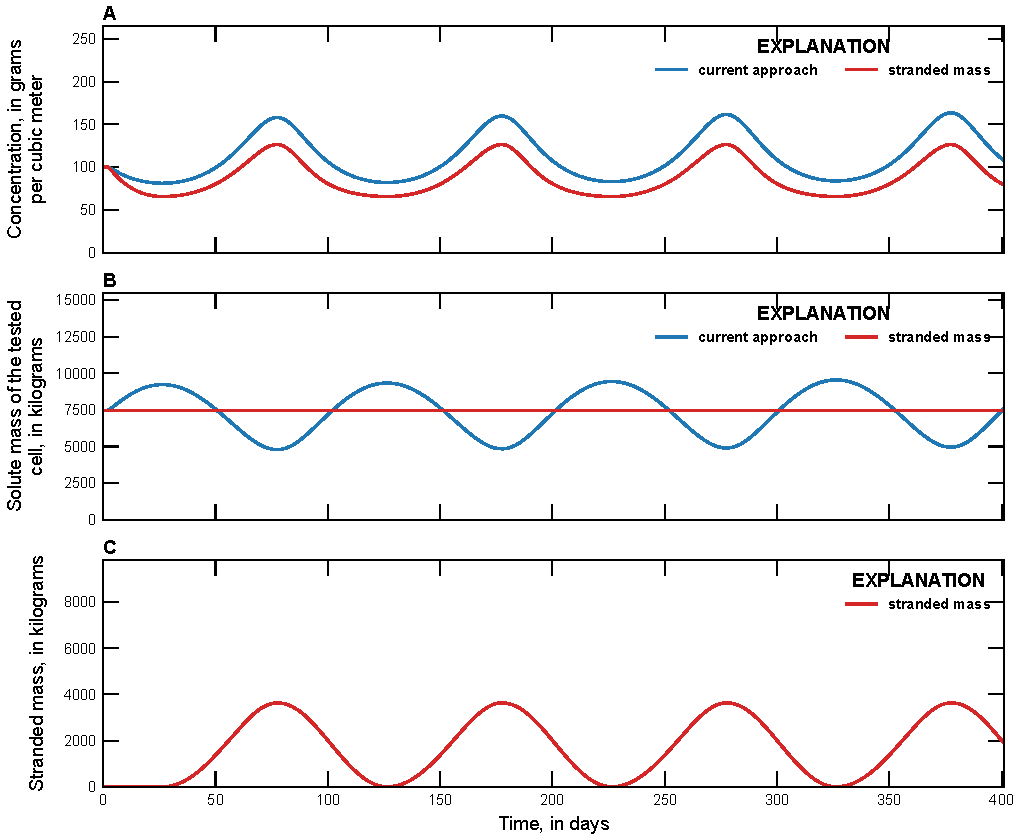
\includegraphics{./Figures/MSTStrandedMassNoSorption.pdf}
	\caption[Graphs comparing simulated concentrations with and without the stranded mass option, without sorption, for the oscillating water table example]{Graphs comparing simulated concentrations with and without the stranded mass option of the MST Package for the oscillating water table example shown in figure~\ref{fig:strandedmasshead}, without sorption and without decay. The cell has a mobile-domain porosity of 0.3, a specific yield of 0.15, and an initial concentration of 100 grams per cubic meter. \textit{A}, Simulated concentration; \textit{B}, solute mass of the tested cell, which is the sum of its dissolved, sorbed, and stranded mass; \textit{C}, stranded mass}
	\label{fig:strandedmassnosorption}
	\end{center}
\end{figure}

Adding sorption (fig.~\ref{fig:strandedmasssorption}\textit{A}) lowers the peak concentration to 146 g/m$^3$, because sorbate buffers the dissolved concentration, and stranded mass lowers it further to 100 g/m$^3$, a reduction of 31 percent, because the sorbate that the cell gives up as it drains is held back along with the solute in the retained water. With first-order decay active, concentrations decrease from cycle to cycle as mass is lost from the simulation, and the concentration at the end of the simulation falls from 14.4 to 9.9 g/m$^3$ with stranded mass. The stranded mass (fig.~\ref{fig:strandedmasssorption}\textit{C}) reaches about 6,780 \si{\kilo\gram} in each cycle without decay, 1.9 times the amount held back when only the retained water contributes, and decreases from cycle to cycle when decay is active, both because the concentration in the cell is lower and because the stranded mass decays while it is held.

The solute mass of the tested cell (fig.~\ref{fig:strandedmasssorption}\textit{B}) ranges between 6,575 and 15,385 \si{\kilo\gram} with sorption and without stranded mass, 77 percent of the mass the cell started with and a wider range than without sorption, because the sorbate that the cell gives up as it drains adds to the solute of the retained water. With stranded mass the same quantity holds at 11,444.4 \si{\kilo\gram}. Decay is the only process that removes solute from the tested cell. With stranded mass the mass of the cell decreases monotonically, from 11,387 to 1,547 \si{\kilo\gram}, as a decaying mass in a closed cell must. Without stranded mass it does not: the mass rises to 13,247 \si{\kilo\gram} during the first cycle, above the 11,387 \si{\kilo\gram} the cell started with, so the drainage and rewetting of the cell create more solute over that cycle than first-order decay removes.

The error without stranded mass grows over a longer simulation. Extended to 40 cycles (4,000 d), the solute mass of the tested cell, compared at the same point of each cycle, is 1.9 percent below the mass the cell started with after the first cycle, 8.6 percent above it after 10 cycles, 21.5 percent after 20, and 52.2 percent after 40, although no solute enters the cell; with sorption it is 7.1, 19.0, and 47.1 percent above after 10, 20, and 40 cycles. The mass created in each cycle grows because it is proportional to the concentration in the cell, which the created mass raises: 127 \si{\kilo\gram} in the 40th cycle without sorption and 177 \si{\kilo\gram} with it. With stranded mass the solute mass of the tested cell is unchanged after 40 cycles.

None of the created mass appears in the model budget. The percent discrepancy of the model budget was 0.00 in every time step of all six simulations in which more than 1 gram per day (g/d) of solute entered or left the model; in the remaining time steps almost no solute moves, and the percent discrepancy is a ratio of numbers near zero.

\begin{figure}[!ht]
	\begin{center}
	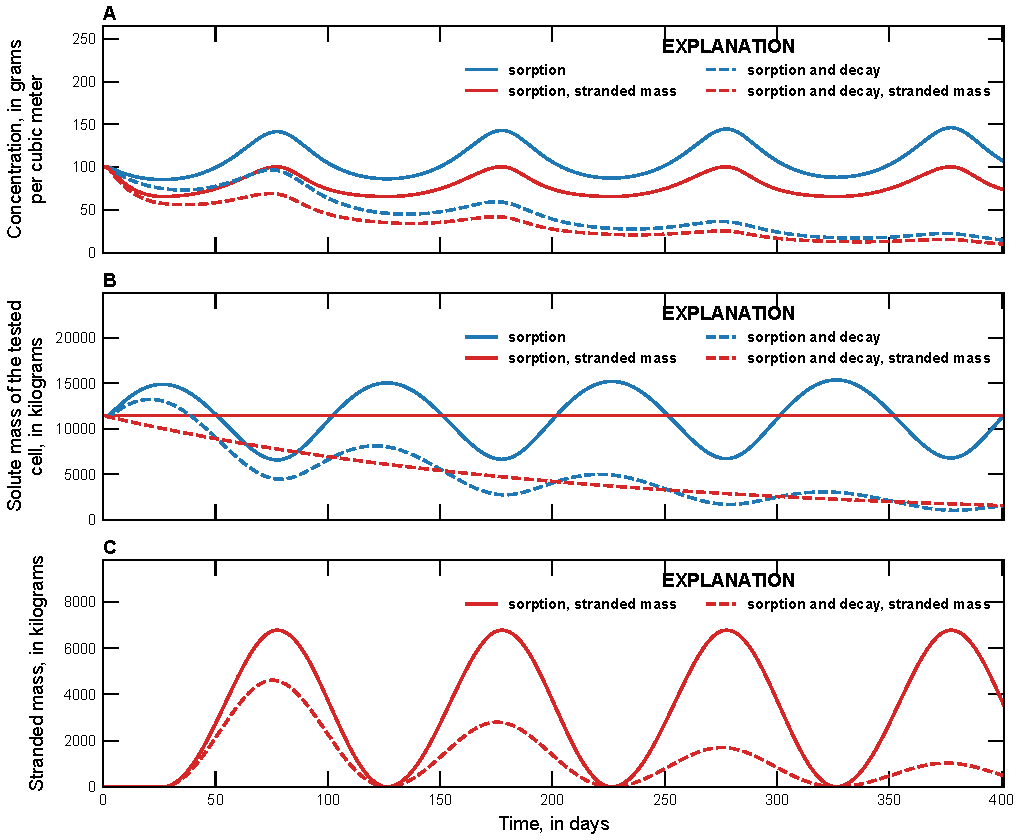
\includegraphics{./Figures/MSTStrandedMassSorption.pdf}
	\caption[Graphs comparing simulated concentrations with and without the stranded mass option, with sorption, for the oscillating water table example]{Graphs comparing simulated concentrations with and without the stranded mass option of the MST Package for the oscillating water table example shown in figure~\ref{fig:strandedmasshead}, with sorption and with sorption and first-order decay. Sorption is represented with a linear isotherm using a bulk density of 1,600 kilograms per cubic meter (kg/m$^3$) and a distribution coefficient of $1 \times 10^{-4}$ cubic meters per kilogram (m$^3$/kg), and the first-order decay rate is 0.005 \si{\per\day} for both the dissolved and the sorbed phase; the remaining properties are the same as those given in figure~\ref{fig:strandedmassnosorption}. \textit{A}, Simulated concentration; \textit{B}, solute mass of the tested cell, which is the sum of its dissolved, sorbed, and stranded mass; \textit{C}, stranded mass}
	\label{fig:strandedmasssorption}
	\end{center}
\end{figure}

\subsection{Sensitivity to Specific Yield and to Sorption}

The size of the effect depends on two quantities, and the oscillating water table example is repeated over a range of each (fig.~\ref{fig:strandedmasssensitivity}). The retained water is the change in the mobile water volume less the water released from storage, so the first quantity is the specific yield relative to the porosity; the simulations that vary it omit sorption so that the retained water is isolated (fig.~\ref{fig:strandedmasssensitivity}\textit{A}). Where the two are equal no mass is stranded, as the formulation requires. As the specific yield decreases, the peak stranded mass rises to 20 percent of the initial mass of the cell at five sixths of the porosity, 49 percent at one half, and 67 percent at one sixth. The departure in concentration from the simulation without stranded mass rises with it at first, to 37 percent of the initial concentration at one half, and then flattens, because the solute held back and the water that would have diluted it are removed together.

The second quantity is the distribution coefficient, and the simulations that vary it hold the specific yield at half the porosity (fig.~\ref{fig:strandedmasssensitivity}\textit{B}). At a distribution coefficient of zero the retained water alone gives 49 percent, and the sorbate adds to it, reaching 67 percent at $4 \times 10^{-4}$ m$^3$/kg. A simulation whose specific yield is close to its porosity and whose solute sorbs weakly is affected little by the option; one whose specific yield was calibrated to reproduce heads, and is well below a measured drainable porosity, is affected strongly.

Without stranded mass, the sign of the error depends on the specific yield relative to the porosity and on how the concentration changes over a cycle. Solute in the retained water leaves the simulation at the concentration of the cell as it drains and is created at the concentration of the cell as it rewets, so the error over a cycle is a gain when the cell rewets at a higher concentration than it drained at, as in the example, and a loss when it rewets at a lower concentration, as when cleaner water enters while the water table rises. Where the specific yield exceeds the porosity, the volume of water inferred for the start of a time step is larger than the volume the mobile domain held, and the sign reverses: with a specific yield of 0.4 and no sorption, the solute mass of the tested cell is 14.5 percent below its starting mass after 10 cycles. With sorption the losses of one part and the gains of the other nearly cancel, and the cell is 0.3 percent below its starting mass after 10 cycles, so a small change in mass does not show that a simulation without stranded mass is free of the error. With stranded mass the solute mass of the tested cell is unchanged in each of these simulations, because the retained water volume is set to zero where the specific yield exceeds the porosity.

\begin{figure}[!ht]
	\begin{center}
	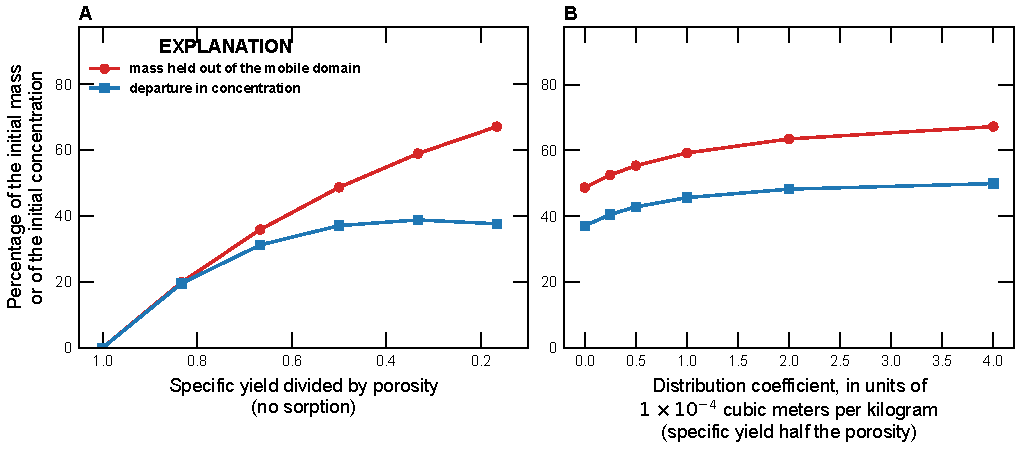
\includegraphics{./Figures/MSTStrandedMassSensitivity.pdf}
	\caption[Graphs showing the sensitivity of the stranded mass option to the specific yield and to the distribution coefficient]{Graphs showing the peak stranded mass, and the peak departure in concentration from a simulation without stranded mass, for the oscillating water table example shown in figure~\ref{fig:strandedmasshead}. Mass is given as a percentage of the mass of the tested cell at the start of the simulation and concentration as a percentage of the initial concentration. \textit{A}, As a function of the specific yield divided by the porosity, without sorption; \textit{B}, as a function of the distribution coefficient, with a specific yield of half the porosity}
	\label{fig:strandedmasssensitivity}
	\end{center}
\end{figure}

\subsection{Example: A Cell That Drains Completely}

The cell of the preceding examples never empties, and a cell that does is treated differently, so a second example lowers the water table below the bottom of the cell and raises it again (fig.~\ref{fig:strandedmassdry}). The cell is the upper of three layers, is 10 \si{\meter} thick, and is drained by a constant head in the lowest layer of the column beside it; the properties are those of the first example, and the first-order rate, where decay is active, is 0.01 \si{\per\day}. The cell is inactive for transport for four of the nine stress periods and has no head and no concentration during them, which is shown as a gap in figures~\ref{fig:strandedmassdry}\textit{A} and~\ref{fig:strandedmassdry}\textit{B}.

The reservoirs keep their mass while the cell is inactive (fig.~\ref{fig:strandedmassdry}\textit{C}). Without decay the stranded mass is unchanged at 2,176 \si{\kilo\gram}, and with decay it falls from 1,572 to 1,165 \si{\kilo\gram}, the first-order decay of a mass that otherwise does not change. Both are returned when the cell is rewet, and both reservoirs are empty once the cell is saturated again, because the time step that reactivates the cell is treated as rewetting.

\begin{figure}[!ht]
	\begin{center}
	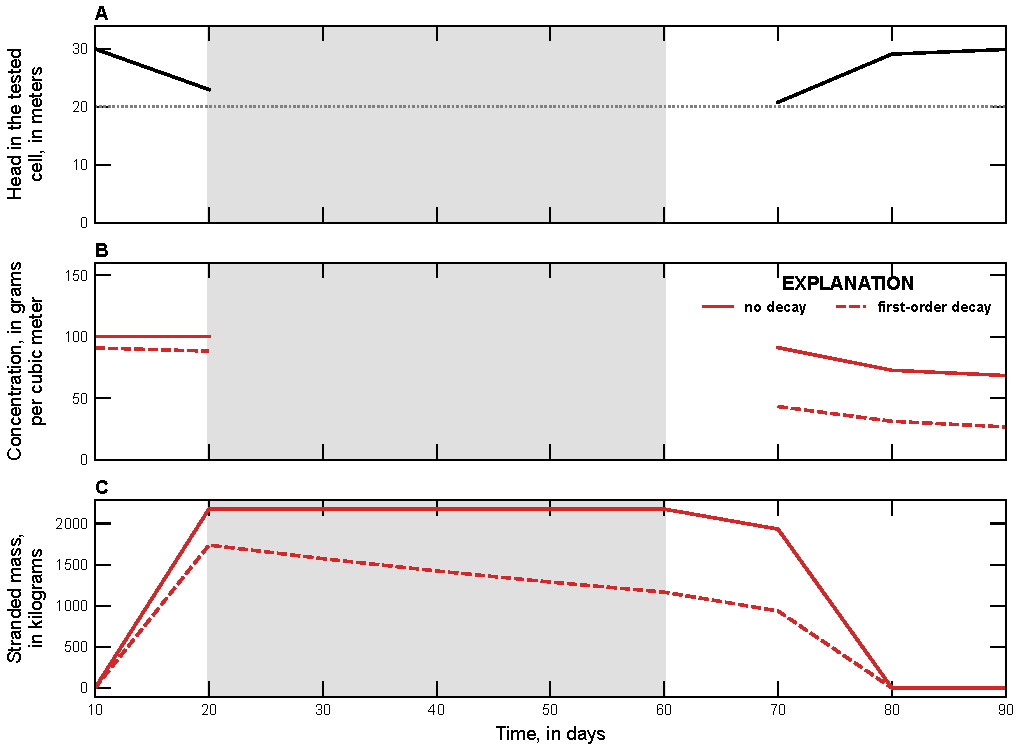
\includegraphics{./Figures/MSTStrandedMassDry.pdf}
	\caption[Graphs showing stranded mass for a cell that drains completely and is later rewet]{Graphs showing the stranded mass of a cell whose water table falls below the bottom of the cell, with and without first-order decay. The cell is inactive for transport over the shaded interval. The dotted line in \textit{A} is the bottom of the cell. \textit{A}, Head in the tested cell; \textit{B}, simulated concentration; \textit{C}, stranded mass}
	\label{fig:strandedmassdry}
	\end{center}
\end{figure}

\subsection{Lakes and Stream Reaches}

The Lake Transport (LKT) and Streamflow Transport (SFT) Packages simulate the solute in a lake or stream reach as a concentration in the water it holds. Evaporation removes water and leaves its solute behind, so the concentration of a lake or reach rises as evaporation reduces its volume. That rise is evaporative concentration, and the STRANDED\_MASS option does not change it, however small the volume becomes. When a lake or reach loses the last of its water, the solute it holds has no water left to be in. Where that water leaves by seepage to the aquifer, through an outlet, to the next reach, by a withdrawal, or through the Water Mover (MVR) Package, it carries the solute with it and nothing is left behind. The problem arises only when a lake or reach goes dry and no water that carries solute leaves it.

That happens in two ways. A lake or reach whose only loss is evaporation can evaporate dry. A stream reach can also go dry when its inflow stops, if the Streamflow Routing (SFR) Package does not route water through reach storage, the default when the STORAGE option is not specified. The depth and volume of such a reach are calculated from the flow through it in each time step, and the water it holds at the end of one time step is not carried into the next. When the inflow stops, that water is not routed downstream or anywhere else, and the volume of the reach is zero in the next time step. The SFT Package does carry the solute of a reach from one time step to the next, so the solute that was in that water remains in a reach that has no water.

Without the option, the concentration of a lake that evaporates dry is undefined, and the simulation stops because the transport solution does not converge. The solute of a reach that goes dry is lost when the reach refills, because the reach refills from a volume of zero, and the SFT budget does not record the loss: it continues to report that solute as stored in the reach. With the option, the solute is held, as the salts that an evaporating water body leaves behind are, and is returned when the lake or reach rewets.

A lake or reach goes dry over a time step when its volume at the end of the time step is zero and no water that carries solute leaves it during the time step. Its solute is then moved to its held mass,

\begin{equation}
\label{eqn:strandapt}
\Delta M_{st} = C \left ( V_0 + V_{in} \right ) ,
\end{equation}

\noindent where $C$ is the concentration of the lake or reach ($M/L^3$), $V_0$ is its volume at the start of the time step ($L^3$), and $V_{in}$ is the volume of water that entered it during the time step ($L^3$). While it is dry, the concentration reported for the lake or reach is that of the water it last held. As the lake or reach rewets, the held mass is returned in proportion to the volume that it regains relative to the volume $V_0 + V_{in}$ that the held mass came from, as in equation~\ref{eqn:strandreturn} with that volume in place of the drained fraction, and all of it is returned once that volume is regained. The held mass is reported as the STRANDED term of the package budget and as the stranded observation, and the option is not available for energy transport.

A lake on an impermeable bed that holds 10,000 cubic meters (m$^3$) of water at 100 g/m$^3$ and evaporates dry over 5 \si{\day} shows the effect for lakes. Without the option, the transport solution fails in the time step in which the lake loses the last of its water. With the option, all 1,000,000 \si{\gram} of solute is held while the lake is dry, three quarters of it is returned when the refilling lake regains 1,500 of the 2,000 m$^3$ that it held at the start of the time step in which it went dry, and the rest is returned in the next time step. The sum of the solute in the lake and the held mass is 1,000,000 \si{\gram} in every time step, and the percent discrepancy of the LKT budget is 0.00 in every time step.

Three reaches in series that exchange no water with the aquifer and do not route water through reach storage show the effect for streams. Each holds 3,857 m$^3$ while water at 100 g/m$^3$ flows through them. After five time steps the inflow stops for five time steps, and then resumes with water that carries no solute. When the inflow stops, the reaches go dry holding 49,989 \si{\gram} of solute, 46,335 \si{\gram} of it in the first reach at 12.0 g/m$^3$. Without the option, the reaches refill at a concentration of zero and that solute is lost, although the SFT budget still reports it as stored. With the option, it is held while the reaches are dry and all of it is returned in the first time step after they refill, when the concentration of the first reach is 11.7 g/m$^3$; the concentration then declines as the inflow flushes the reach.

\subsection{Assessment}

The formulation conserves mass by construction. The mobile domain loses exactly the mass that the reservoirs gain and gains exactly the mass that they lose, so the sum of the mobile and stranded mass changes only through decay and the flows across the boundaries of the model. No mass is averaged in from neighboring cells, adjusted, or discarded, so a discrepancy in the model budget would indicate an error in the program rather than a modeling choice. The approaches available in MT3D-USGS \citep{mt3dusgs} do not have this property: a cell that rewets is assigned either an inverse-distance-weighted average of the concentrations of its neighbors, which creates mass, or a concentration of zero, which destroys it.

The formulation is an approximation in five respects.

\begin{itemize}

\item \textbf{The unsaturated zone is not simulated.} The stranded mass is held in place and returned when the cell rewets. It does not move, so solute cannot be carried downward through the unsaturated zone by infiltrating water, and it cannot be redistributed within the drained interval. A simulation that needs those processes should represent the unsaturated zone explicitly with the Unsaturated Zone Flow (UZF) Package and the Unsaturated Zone Transport (UZT) Package, which requires considerably more input.

\item \textbf{Sorbate is held out of equilibrium.} Sorbate in the drained interval is assumed to keep the mass it had when the interval drained. In reality the solid aquifer material above the water table remains in contact with the retained water, and the sorbed and dissolved phases of that water continue to interact. Holding the mass unchanged is defensible when the retained water is nearly immobile and its contact with the mobile domain is slight, and becomes less so as the drained interval becomes wetter.

\item \textbf{The retained water is taken from the specific yield.} The retained water is the difference between the change in the mobile water volume and the water released from storage, so it is whatever the porosity of the transport model and the specific yield of the flow model imply. The two models cannot disagree about it and no value has to be estimated, but a simulation whose specific yield was calibrated to reproduce heads, rather than measured as a drainable porosity, carries that choice into the simulated concentrations. Specific yield is the drainable part of the pore space and cannot exceed the porosity, but the two are independent inputs to two different models. Where the specific yield is the larger of the two, the flow model releases more water from storage than the mobile domain holds, no solute is retained in those cells, and a warning is written to the simulation listing file; the sorbate is stranded as usual and mass is conserved either way. A flow model solved in the same simulation always supplies the storage flow that the retained water is computed from, but a transport model that reads the flows saved by a separate flow simulation needs the specific yield storage flow (STO-SY), which the flow model saves only if SAVE\_FLOWS is specified in its Storage Package or its name file. Without it the drained pore volume would be treated as entirely retained, which is the result a specific yield of zero would give, so the option terminates with an error rather than running.

\item \textbf{The unsaturated zone packages are not accounted for.} The UZF and UZT Packages represent the drained interval explicitly, and the MST Package does not account for them. A simulation that uses UZF and UZT together with this option represents the same drained interval twice, once as water and solute moving through the unsaturated zone and once as stranded mass, and the two representations do not agree: UZT has no sorbed phase and no decay, whereas the stranded mass has both. The option is intended for simulations that do not represent the unsaturated zone explicitly, and it should not be used together with UZT. A model in which both are active is reported with a warning rather than refused, because the UZF Package often covers only part of a model and stranded mass is meaningful in the cells that it does not cover.

\item \textbf{The distribution within the drained interval is uniform.} The share of the stranded mass that returns is proportional to the share of the drained interval that rewets. A water table that falls slowly and rises quickly, or a cell that is thick relative to the range of the water table, returns mass in a different order than a model that resolved the vertical distribution would.

\end{itemize}

The option is intended for simulations in which the water table moves through cells that have a substantial sorbed mass or a specific yield well below the porosity, in which redissolving that mass or losing the solute of the retained water on drainage is a recognized artifact, and in which representing the unsaturated zone explicitly is not warranted. Under those conditions it removes an artifact of the storage formulation without introducing a term that has to be calibrated: the stranded mass is determined by the specific yield and the sorption parameters that the simulation already uses, and the option has no effect when the specific yield equals the porosity and sorption is not active.

\subsection{Relation to MT3D-USGS}

Alternative treatments of the sorbed mass of a cell whose water table moves are compared by Bedekar and others (V. Bedekar, S.S. Papadopulos \& Associates, Inc., written communication, 2021). MT3D-USGS \citep{mt3dusgs} revised the storage formulation of MT3DMS so that the sorbed part of the storage term is accumulated in a reservoir for the cell rather than released to the water that remains, and is returned when the cell rewets in proportion to the share of the unsaturated volume of the cell that resaturates; the earlier formulation remains available through the LEGACY99STORAGE keyword of the Basic Transport Package. The sorbed half of the formulation described in this chapter is the same idea expressed in the terms of the MODFLOW~6 transport models.

The formulation described here differs in four respects.

\begin{itemize}

\item \textbf{Solute in the retained water is held back as well.} MT3D-USGS releases the dissolved part of the storage term in full at the concentration of the previous time step, so the solute in the retained water is lost. That formulation has no retained water, because the water released from storage and the change in the mobile water volume are assumed to be the same quantity.

\item \textbf{The stranded mass decays.} Mass held out of the mobile domain by MT3D-USGS is inert for as long as it is held, so a cell that stays dry for a long time returns the mass it started with. Here each reservoir decays at the rate given for its phase, which matters when the period between drainage and rewetting is long relative to the half-life.

\item \textbf{The share that returns is measured relative to the drained interval.} MT3D-USGS returns the reservoir in proportion to the share of the unsaturated volume of the cell that resaturates, so the mass held back from a small fall of the water table is spread over the whole unsaturated part of the cell. Bedekar and others (written communication, 2021) note that this underestimates the mass returned when the water table moves through only a small part of a cell. Here the share is measured relative to the drained fraction $F$ of equation~\ref{eqn:strandreturn}, the part of the cell that drained while the mass was held. A cell that drains from a saturation of 0.5 to 0.3 and rewets to 0.4 recovers half of its stranded mass here and one seventh of it in MT3D-USGS.

\item \textbf{The behavior is optional.} MT3D-USGS applies its formulation unless the legacy formulation is requested, whereas the formulation described here is active only when the STRANDED\_MASS option is specified, so existing simulations are unaffected.

\end{itemize}

The retained water term removes the assumption that the water released from storage equals the change in the mobile water volume. MT3D-USGS recovers the volume of water in the cell at the end of the previous time step by dividing the flow to storage by the porosity, which is exact only when the drainable porosity and the porosity are the same. The transport models of MODFLOW~6 obtain that volume by adding the flow to storage directly, which makes the same assumption. Specific yield is the drainable part of the pore space and is ordinarily smaller than the porosity, so the difference between the two is the retained water, and the formulation described in this chapter uses that volume, rather than a value the user supplies, to determine how much solute is held back. Bedekar and others (written communication, 2021) note that a storage formulation that assumes the two volumes are the same gives meaningful results only when the specific yield equals the porosity, and that a porosity greater than the specific yield requires the water between the two to be treated separately, as \citet[eq.~26]{panday2008} do.
